\documentclass[12pt, openright, oneside]{report}
% Language and encoding
\usepackage[utf8]{inputenc}
\usepackage[english]{babel}
% Page layout and margins
\usepackage[a4paper, margin=1in]{geometry}
% Graphics and captions
\usepackage{graphicx}                 % For including images
\usepackage{subcaption}               % For subfigures (if needed)
\usepackage[labelfont=bf, figurename=Fig., tablename=Table, font=small]{caption}
\captionsetup{font={small, stretch=1.2}} 
\usepackage[table,xcdraw]{xcolor}
\usepackage{makecell} % Literally just to have the command '\Xhline' in a table, i hate this
% Math and symbols
\usepackage{amsmath} % For advanced math commands
\usepackage{amssymb} % For additional symbols
\usepackage{bbold}   % For bold mathematical symbols
% References
\usepackage[backend=biber, sorting=none]{biblatex} % For references
\addbibresource{references.bib}                     % Point to your bibliography file
% Title and section formatting
\usepackage{titlesec}
\titleformat{\section}{\normalfont\Large\bfseries}{\thesection}{1em}{}
\titleformat{\subsection}{\normalfont\large\bfseries}{\thesubsection}{1em}{}

% Lists and tables
\usepackage{enumitem} % For custom lists
\usepackage{multirow} % For tables with merged rows
\usepackage{multicol} % For multi-column text (if needed)
% Typography improvements
\usepackage{microtype} % Improves text justification and spacing
% Custom margins for specific content
\usepackage{changepage} % To change margins for specific sections (e.g., images)
% Floating objects
\usepackage{float} % For precise positioning of floats
% Miscellaneous
\usepackage{comment}  % To comment out large blocks of text
% TikZ and PGFPlots (if needed for graphs)
\usepackage{tikz}     % For custom graphics
\usepackage{pgfplots} % For plots and charts
\pgfplotsset{compat=1.18}
% Reduce compilation time (useful for TikZ-heavy documents)
\usepgfplotslibrary{external}
\tikzexternalize
% Line spacing
\renewcommand{\baselinestretch}{1.5}
% Footnote line spacing
\setlength{\footnotesep}{0.8\baselineskip} 
% Headers and footers (if customization is needed)
\usepackage{fancyhdr}
% Replace "Chapter" with "Assignment" and enforce vertical layout
\titleformat{\chapter}[display] % Display style ensures vertical layout
  {\normalfont\huge\bfseries} % Formatting for the title
  {Assignment \thechapter} % Replace "Chapter" with "Assignment"
  {0pt} % No space between "Assignment [n]" and the vertical space
  {\vspace{1em}} % Vertical space before the chapter title

% Configure the fancy header
\pagestyle{fancy}
\fancyhf{} % Clear all header and footer fields
\fancyhead[L]{M. Arrighini, L. Babiski Arruda, G. Cottini, E. Paciaroni} % Authors in the top-left corner
\fancyhead[R]{} % Assignment number in the top-right corner
\fancyfoot[C]{\thepage} % Page number centered in the footer
\renewcommand{\headrulewidth}{0.4pt} % Adds a horizontal line to the header

\usepackage{lmodern} % Use Latin Modern scalable fonts
\definecolor{unired}{RGB}{176,0,0}
% Hyperlinks
\usepackage{hyperref}
\hypersetup{
    colorlinks=true,
    linkcolor=blue,
    filecolor=magenta,
    urlcolor=cyan,
    pdftitle={Group Project Report},
    pdfpagemode=FullScreen,
}

\begin{document}

%-------- Title page -------------------------------------------------------------------------------------------------------%

    \begin{titlepage}
        \centering
        
\includegraphics[width=0.3\textwidth]{images/logo_unipd.png}\par\vspace{1cm}
        {\scshape\LARGE Università degli Studi di Padova \par}
        \vspace{1.5cm}
        {\scshape\Large Master Degree Course in Computational Finance \par}
        \vspace{.2cm}
        {\scshape\large Regression and Time Series Models \par}
        \vspace{2cm}
        {\Large\bfseries Group Work 1 - Regression with CAPM Model\par}
        \vspace{2cm}
        Created by:\par
        {\itshape{Martina Arrighini, 2149799, martina.arrighini@studenti.unipd.it}\par}
        {\itshape{Luigi Babiski Arruda, 2163341, luigi.babiskiarruda@studenti.unipd.it}\par}
        {\itshape{Giorgio Cottini, 2140740, giorgio.cottini@studenti.unipd.it}\par}
        {\itshape{Enrico Paciaroni, 2139678, enrico.paciaroni@studenti.unipd.it}\par}
        \vfill
        Commissioned by:\par
        Prof.\ Massimiliano Caporin
        \vfill
        {\large A.Y. 2024/2025}
    \end{titlepage}

% Start counting pages
\setcounter{page}{1}

%-------- Table of Contents ------------------------------------------------------------------------------------------------%
\tableofcontents

%-------- Overview ---------------------------------------------------------------------------------------------------------%
\chapter*{Overview}
This report analyzes the Healthcare sector within the Euro Stoxx 600 index, using data from October 2000 to October 2024 to
evaluate the applicability of the Capital Asset Pricing Model (CAPM). 
The Healthcare sector, known for its inelastic demand, high entry barriers, and resilience, provides a compelling context for 
assessing risk-return dynamics.

Using Ordinary Least Squares (OLS) regression, we estimate CAPM parameters, including alpha, beta, and R-squared, for both 
individual equities and an equally weighted portfolio. Diagnostic tests, such as the White and Breusch-Godfrey tests, ensure 
the robustness of the model. Additionally, a multifactor model based on the Fama-French framework is introduced to compare its
explanatory power with that of the CAPM.

Structural breaks in the data are analyzed using the Chow test and a rolling window approach, providing insights into 
parameter stability over time. This collaborative effort aims to deliver a comprehensive evaluation of the CAPM and 
multifactor models, offering valuable insights into the financial dynamics of the Healthcare sector.
%-------- Assignment 1 -----------------------------------------------------------------------------------------------------%
\chapter{Data Choice and Download}
In this assignment, we gathered and prepared the necessary data for analyzing the Healthcare sector within the Euro Stoxx 600
index. 
The data includes total return indices for individual stocks, risk-free interest rates, and the market index for the
healthcare sector.

\section{Data Collection}
\begin{itemize}
    \item \textbf{Total Return Indices:} We obtained the total return indices for ten companies within the Healthcare sector.
    These companies were selected based on the availability of complete data from 2000 to 2024.
    \item \textbf{Market Index:} The Euro Stoxx 600 Health Care index was used as a benchmark for the overall market performance
    within the sector.
    \item \textbf{Risk-Free Rates:} Monthly risk-free interest rates were derived from annualized Federal Reserve data to
    compute excess returns.
\end{itemize}

\section{Data Preparation}

\begin{itemize}
    \item \textbf{Return Calculation:} Monthly returns were calculated using logarithmic differences in prices. This method 
    ensures that the data is approximately normally distributed and facilitates economic interpretation.
    \item \textbf{Excess Returns:} Stock and market returns were adjusted by subtracting the risk-free rate, consistent with the 
    CAPM framework.
    \item \textbf{Data Quality Checks:} The datasets were thoroughly examined for missing or duplicate values to ensure the 
    robustness of subsequent analyses.

\end{itemize}

\section{Preliminary Visualization}
Scatter plots were created to examine the relationship between stock excess returns and market excess returns. 
These plots showed a clear linear relationship for most equities, supporting the applicability of the CAPM. 
However, some observations indicated potential outliers, which will be analyzed further in later steps.\label{chapter:download}

%-------- Assignment 2 -----------------------------------------------------------------------------------------------------%
\chapter{Relationship Between Stock and Market Returns}\label{chapter:equity_returns}
In this section, we analyze the relationship between the excess returns of individual stocks and those of the sector market
using scatter plots.
The objective is to explore whether linear relationships exist, as assumed by the CAPM model. 
Scatter plots are used to visually assess the correlation between variables and to identify potential deviations.
Particular focus is given to outliers and non-linear trends, as these could suggest the need for deeper analysis or
alternative approaches.
The scatter plots reveal a clear relationship between the excess returns of most stocks and the sector market.
For instance, stocks like Johnson \& Johnson, Pfizer, and Medtronic show a well-defined linear trend, indicating a strong 
correlation with market returns. 
These results suggest that the CAPM model can effectively describe the variability in returns for these stocks, supported by
significant $\beta$ coefficients and high R² values.
However, some stocks, such as Boston Scientific and Cigna, display more scattered data points around the trendline, 
pointing to weaker correlations and the influence of unique factors that the CAPM might not capture.
In addition, outliers observed in stocks like Revvity and Labcorp Holdings could reflect extraordinary events, such as 
regulatory changes or R\&D results, which may reduce the model's effectiveness for these cases.
The slope of the trendline offers further insights: for example, Eli Lilly and Teleflex demonstrate steeper slopes,
suggesting a high $\beta$ and greater sensitivity to market movements, while flatter slopes, as observed in Humana, indicate lower 
exposure to systematic risk.
Overall, our observations suggest that the CAPM model effectively explains the behavior of most stocks analyzed. 
However, instances of high dispersion or the presence of significant outliers underscore the need for further evaluation, 
which will be undertaken in subsequent stages of the analysis.


\begin{figure}[h]
    \centering
    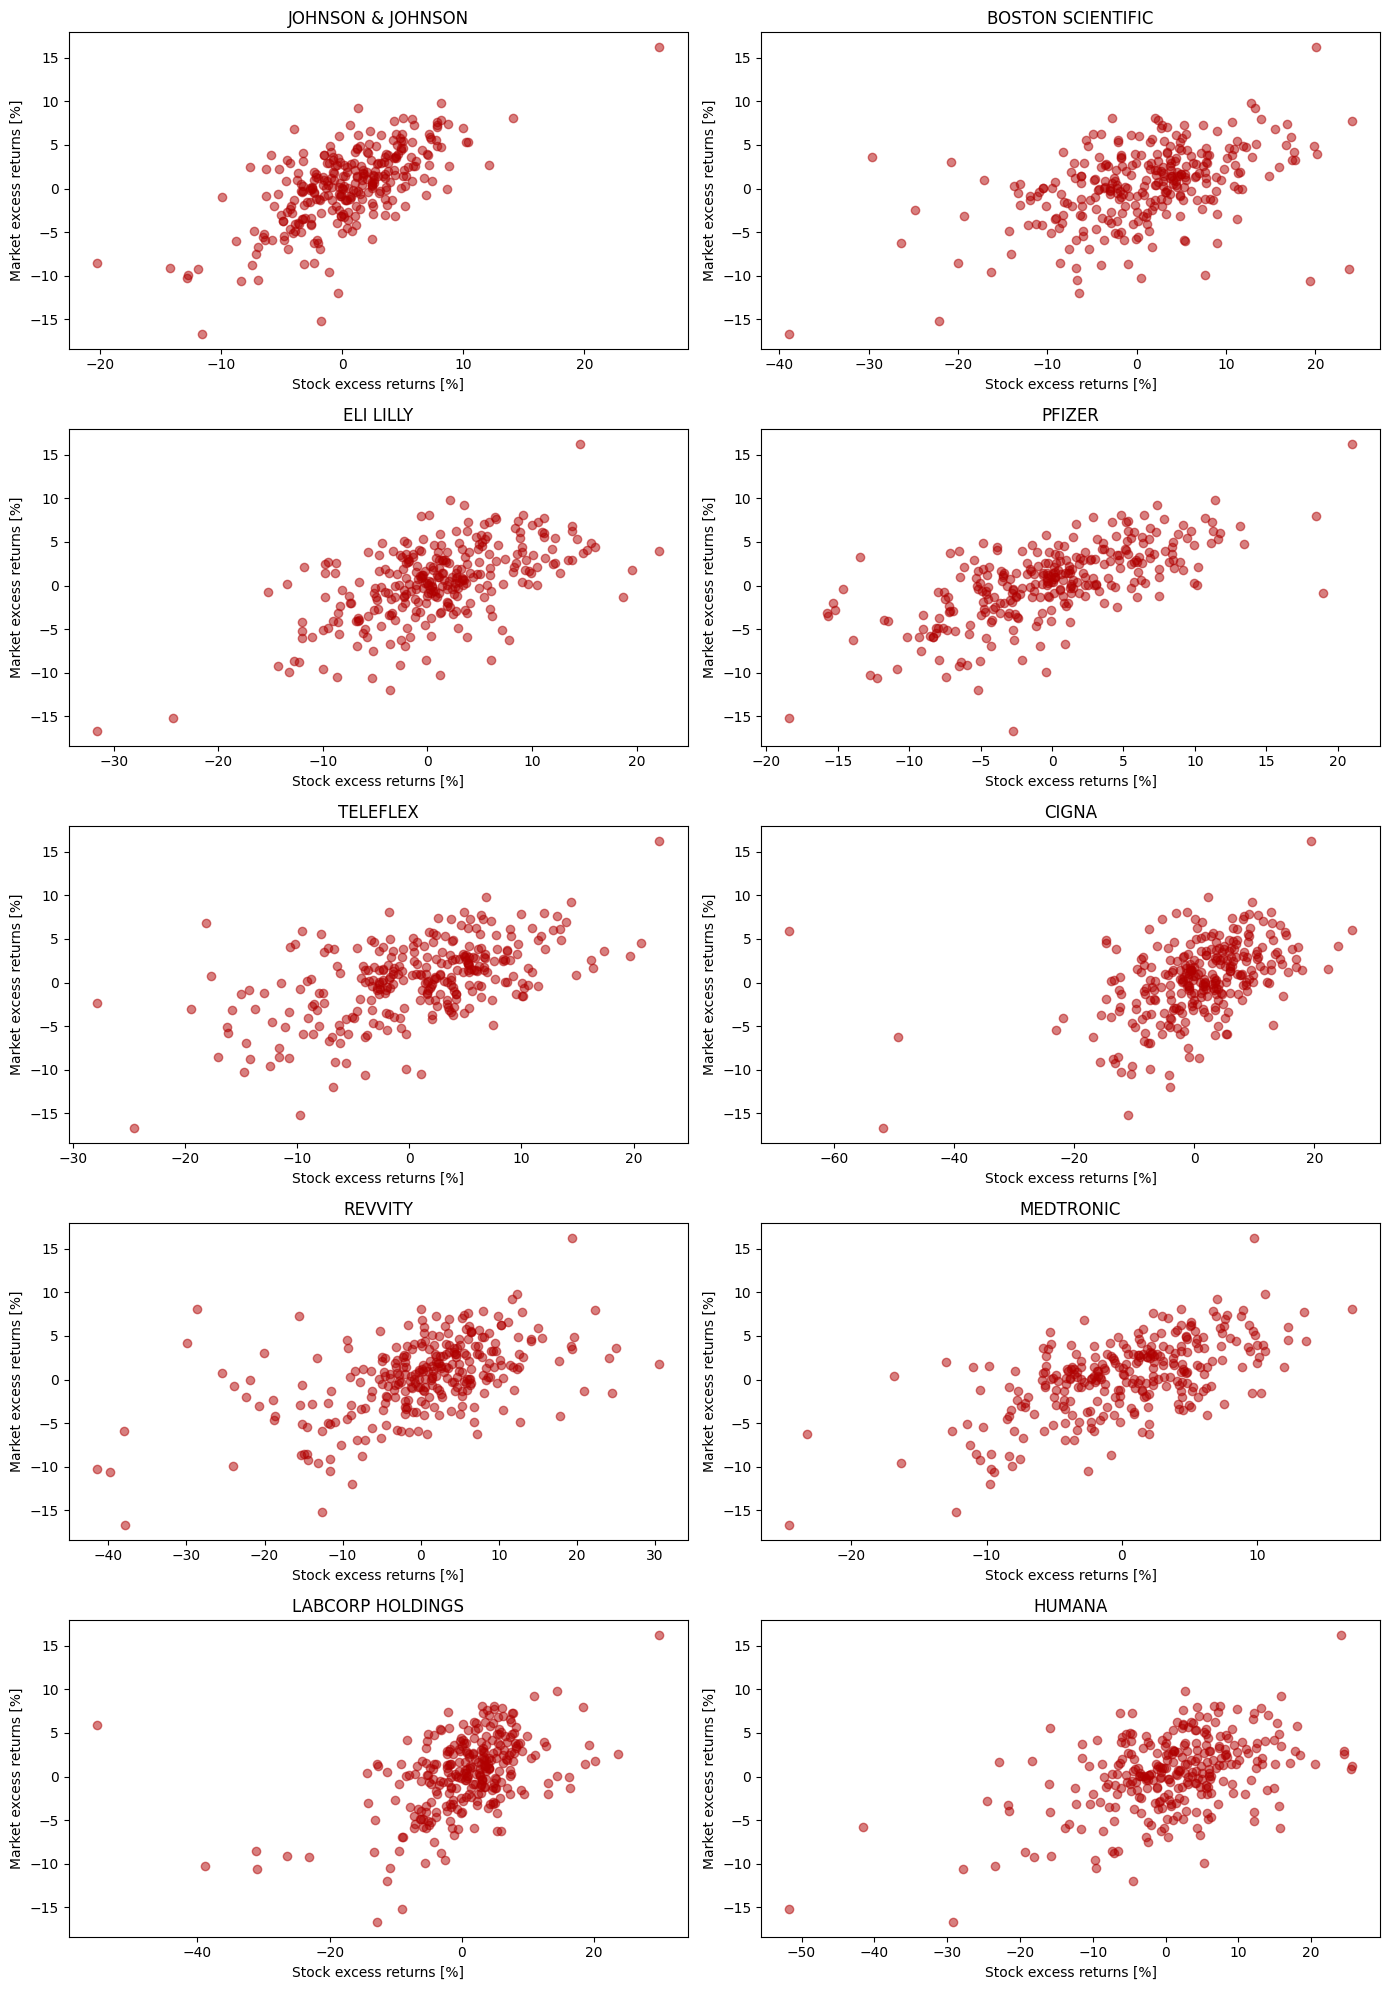
\includegraphics[width=0.8\textwidth]{images/equities_scatterplot.png}
    \caption{Scatterplot of equities' log-returns against excess market returns.}\label{fig:equities_scatterplot}
\end{figure}

%-------- Assignment 3 -----------------------------------------------------------------------------------------------------%
\chapter{CAPM Regression}\label{chapter:linear_regression}
\section{Regression Results for Individual Stocks}

The CAPM regression applied to individual stocks highlights significant findings regarding $\alpha$, $\beta$ and $R^2$ values 
(see Table~\ref{tab:regression_results} for reference).
Stocks like Johnson \& Johnson and Pfizer exhibit high $\beta$ coefficients, indicating a strong sensitivity to market
movements, with market returns explaining a substantial portion of their variability. These results confirm the applicability 
of the CAPM model to these stocks and its ability to estimate systematic risk effectively.
However, not all stocks perform equally well under the CAPM framework. Stocks like Cigna and Labcorp Holdings show relatively
low $R^2$ values, indicating that a smaller proportion of their return variability is explained by market factors. 
This suggests the presence of idiosyncratic risks or company-specific drivers that are not captured by the model. 
These discrepancies highlight the limitations of CAPM in explaining returns for stocks with unique business models or exposure 
to niche markets.
For stocks with lower $R^2$ values, alternative approaches, such as incorporating additional explanatory variables 
(e.g., size, value, or momentum factors), may enhance model reliability. 
These findings suggest that while the CAPM model provides a robust foundation for analyzing systematic risk, its assumptions
may need to be adjusted for certain stocks.

\begin{table}[htbp]
    \centering
    \footnotesize
    \renewcommand{\arraystretch}{1.2} % Adjust row height
    \begin{tabular}{|l|c|c|c|c|c|c|c|}
        \hline
        \rowcolor{unired!30} \textbf{Company} & \textbf{$\alpha$} & \textbf{$\beta$} & \textbf{$R^2$} & \textbf{Err. $\alpha$} & \textbf{Err. $\beta$} & \textbf{$\Delta \beta$ [0.025]} & \textbf{$\Delta \beta$ [0.975]} \\ \hline
        Johnson \& Johnson & 0.2451 & 0.7474 & 0.455 & 0.212 & 0.048 & 0.652 & 0.843 \\ \hline
        \rowcolor{gray!10} Boston Scientific & 0.3464 & 0.9036 & 0.207 & 0.458 & 0.105 & 0.698 & 1.109 \\ \hline
        Eli Lilly & 0.5655 & 0.9314 & 0.342 & 0.335 & 0.076 & 0.781 & 1.082 \\ \hline
        \rowcolor{gray!10} Pfizer & -0.3246 & 0.9595 & 0.451 & 0.274 & 0.063 & 0.836 & 1.083 \\ \hline
        Teleflex & 0.3055 & 0.9621 & 0.297 & 0.383 & 0.088 & 0.790 & 1.134 \\ \hline
        \rowcolor{gray!10} Cigna & 0.2511 & 1.0512 & 0.212 & 0.525 & 0.120 & 0.815 & 1.287 \\ \hline
        Revvity & -0.2457 & 1.2225 & 0.265 & 0.527 & 0.120 & 0.985 & 1.460 \\ \hline
        \rowcolor{gray!10} Medtronic & -0.1108 & 0.8613 & 0.384 & 0.282 & 0.065 & 0.734 & 0.988 \\ \hline
        LabCorp Holdings & 0.2675 & 0.9163 & 0.233 & 0.430 & 0.098 & 0.723 & 1.110 \\ \hline
        \rowcolor{gray!10} Humana & 0.5939 & 1.0700 & 0.231 & 0.506 & 0.116 & 0.843 & 1.298 \\ \Xhline{1.2\arrayrulewidth}

        \textbf{Portfolio} & \textbf{0.2234} & \textbf{0.8677} & \textbf{0.772} & \textbf{0.122} & \textbf{0.028} & \textbf{0.813 } & \textbf{0.923} \\ \hline
    \end{tabular}
    \caption{Regression results for each company, detailing Alpha, Beta, R-squared, and confidence intervals.}
    \label{tab:regression_results}
\end{table}

\section{Performance of the Weighted Portfolio}
The weighted portfolio demonstrates a strong alignment with the CAPM model, as evidenced by its significant and consistent
$\beta$ coefficient and high $R^2$ values. 
The compact and regular distribution of data points around the regression line highlights the effectiveness of diversification 
in reducing idiosyncratic risks and enhancing the model's explanatory power. 
This finding underscores the stability of portfolio returns when individual stock-specific risks are averaged out.
Compared to individual stocks, the portfolio benefits from a smoother relationship with market returns, as diversification 
minimizes the noise caused by unique company events. This results in more reliable estimates of $\beta$ and a higher goodness 
of fit ($R^2$), confirming the portfolio's sensitivity to systematic risk.
These characteristics make the CAPM model particularly suitable for analyzing aggregate portfolio behavior.
The portfolio's performance under the CAPM model reinforces the importance of diversification as a strategy for mitigating
risk and achieving more predictable returns. 
By averaging out the effects of outliers and company-specific shocks, the portfolio provides a clearer view of systematic 
risk and market sensitivity.

\begin{figure}[h]
    \centering
    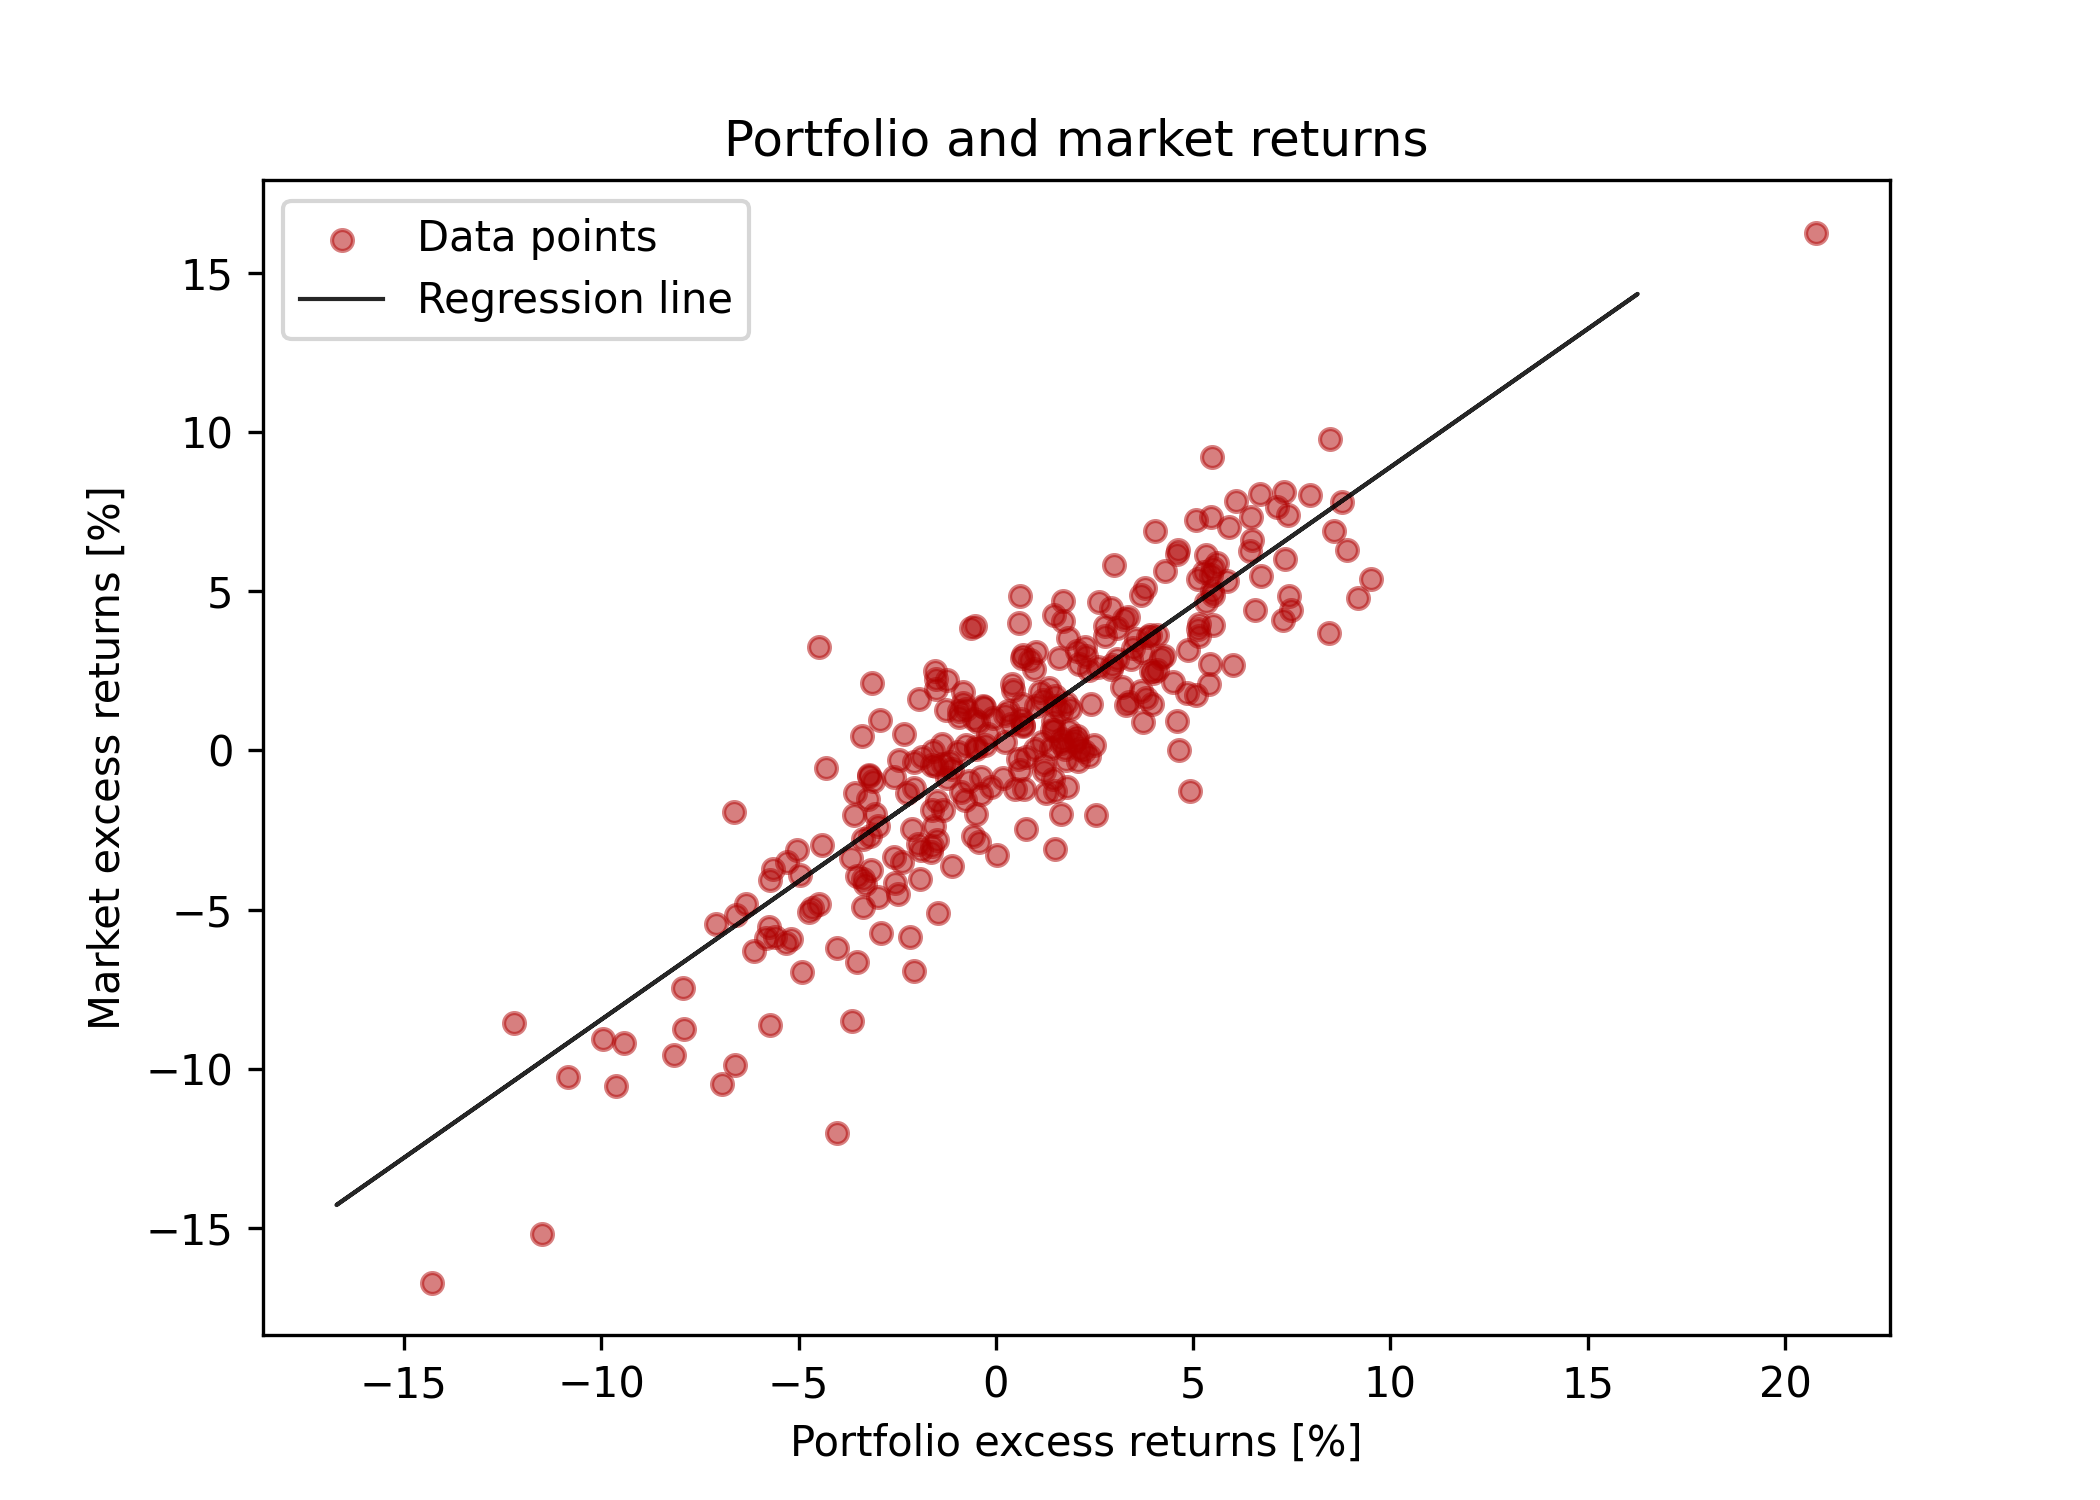
\includegraphics[width=0.8\textwidth]{images/portfolio_regression.png}
    \caption{Scatterplot of portfolio's returns against excess market returns, with linear regression.}\label{fig:portfolio_regression}
\end{figure}

\section{Impact of Diversification}
Diversification proves to be a key factor in stabilizing the parameter estimates of the CAPM model. 
While individual stocks may exhibit high variability in $\beta$ and $\alpha$ due to idiosyncratic risks, the equally weighted
portfolio achieves greater consistency. 
This is particularly evident in its reduced residual variance and higher $R^2$ values, which indicate a stronger fit to the 
CAPM framework.
The ability of diversification to average out company-specific risks highlights its role in improving the reliability of 
financial models. 
For investors, this suggests that constructing diversified portfolios can lead to more predictable risk and return profiles,
even when individual stocks deviate from expected patterns. 
Diversification also reduces the influence of outliers, providing a clearer picture of systematic risk.
These observations underscore the practical applications of the CAPM model for portfolio analysis, where diversification
enhances its explanatory power. 
However, the model's limitations in capturing unique factors for individual stocks emphasize the need for supplemental
analyses when evaluating less diversified assets.


%-------- Assignment 4 -----------------------------------------------------------------------------------------------------%
\chapter{Diagnostic Tests}\label{chapter:diagnostic_tests}
\section{Significance of $\beta$ and $R^2$ Values}
The results of the CAPM regression, displayed in Table~\ref{tab:equity_results}, confirm the model's ability to explain the 
returns of many stocks. 
Stocks like Johnson \& Johnson ($\beta$=0.752, $R^2$=0.458) and Pfizer ($\beta$=0.953, $R^2$=0.449) exhibit significant
$\beta$ coefficients and high $R^2$ values, indicating strong sensitivity to market movements. 
These results validate the CAPM model's assumption that systematic risk is the primary driver of returns for these stocks.
However, stocks with lower $R^2$ values, such as Cigna and Labcorp Holdings, suggest the presence of significant idiosyncratic 
risks or external factors that are not captured by the CAPM framework.
These findings emphasize the model's limitations when applied to companies influenced by unique events or niche market 
dynamics.
To improve the model's accuracy for such cases, additional factors, such as industry-specific risks or macroeconomic
variables, could be incorporated. 
This would help account for variability that the CAPM model alone cannot explain, particularly for stocks with lower market 
correlations.

\begin{table}
    \centering
    \renewcommand{\arraystretch}{1.2} % Adjust row height
    \footnotesize
    \begin{tabular}{|l|c|c|c|c|c|c|}
        \hline
        \rowcolor{unired!30} \textbf{Equity} & \textbf{$\beta$} & \textbf{$\beta$ p-value} & \textbf{White p-value} & \textbf{BG p-value} & \textbf{$R^2$} & \textbf{HAC p-value} \\ \hline
        Johnson \& Johnson & 0.752 & 0 & 7.19E-10 & 0.178 & 0.458 & 0.001 \\ \hline
        \rowcolor{gray!10} Boston Scientific & 0.91 & 0 & 2.17E-05 & 0.846 & 0.21 & 0.003 \\ \hline
        Eli Lilly & 0.942 & 0 & 0.013 & 0.085 & 0.346 & 0.009 \\ \hline
        \rowcolor{gray!10} Pfizer & 0.953 & 0 & 0.209 & 0.094 & 0.449 & 0.008 \\ \hline
        Teleflex & 0.968 & 0 & 0.921 & 0.762 & 0.3 & 0.010 \\ \hline
        \rowcolor{gray!10} Cigna & 1.056 & 0 & 0.119 & 0.988 & 0.214 & 0.015 \\ \hline
        Revvity & 1.218 & 0 & 0.130 & 0.999 & 0.265 & 0.020 \\ \hline
        \rowcolor{gray!10} Medtronic & 0.859 & 0 & 0.477 & 0.192 & 0.384 & 0.012 \\ \hline
        Labcorp Holdings & 0.921 & 0 & 0.207 & 8.85E-07 & 0.236 & 0.005 \\ \hline
        \rowcolor{gray!10} Humana & 1.081 & 0 & 2.87E-05 & 0.989 & 0.235 & 0.014 \\ \hline
    \end{tabular}
    \caption{Regression results for each equity, including Beta, p-values, and various test results.}
    \label{tab:equity_results}
\end{table}

\section{Heteroscedasticity Issues}
The White Test identifies heteroscedasticity in stocks such as Johnson \& Johnson and Humana, indicating non-constant residual variance. This violation of CAPM assumptions suggests that the reliability of the regression results may be compromised, as standard errors may be underestimated or overestimated.
To address this issue, robust standard errors (HAC) were applied, which adjust for heteroscedasticity and provide more reliable parameter estimates. These adjustments ensure that the significance levels of $\beta$ coefficients remain valid despite violations of homoscedasticity.
Future analyses could explore whether specific periods or events contribute to heteroscedasticity. Understanding these patterns may help refine the CAPM model's application to stocks affected by irregular variance in their residuals.

\section{Autocorrelation in Residuals}
The Breusch-Godfrey Test detects autocorrelation in stocks such as Labcorp Holdings, suggesting that the residuals are not 
independently distributed.
This violates the CAPM assumption of no autocorrelation, which can lead to biased parameter estimates and reduced model 
reliability.
To mitigate the impact of autocorrelation, adjustments such as incorporating lagged variables or alternative error correction
methods can be applied. 
These techniques improve the robustness of the regression results and enhance the reliability of the CAPM model for stocks 
with autocorrelated returns.
Despite these challenges, the CAPM model remains effective for analyzing diversified portfolios.
The reduction of idiosyncratic risks and the alignment of residuals with model assumptions further support its applicability 
at an aggregate level.
However, for individual stocks with significant deviations, additional diagnostic tools and model refinements are necessary to 
ensure accurate analysis.

%-------- Assignment 5 -----------------------------------------------------------------------------------------------------%
\chapter{Chow Test}\label{chapter:chow_test}
\section{Structural Breaks and Chow Test}

In this section, we employ the Chow test to assess whether a significant structural change occurs in the regression models at 
specific points in time. 
To ensure the robustness of our analysis, we first established a minimum data subset size for the unrestricted models, 
setting it to 10\% of the total dataset, in order to maintain statistical validity while preserving sufficient data for
meaningful comparisons.
Subsequently, the Chow test was systematically applied to all linear regressions conducted on the selected equities, 
allowing us to identify potential structural breaks across the dataset, that is, significant changes in the regression
parameters caused by external shocks, market-wide events, or company-specific factors. 
Structural breaks may reflect changes in the relationship between excess returns and market behavior, such as shifts in 
systematic risk $(\beta)$ or unexplained excess returns $(\alpha)$, driven by macroeconomic conditions,
regulatory adjustments, or sector developments.
Structural breaks were identified by analyzing the p-values from the Chow test over time: a p-value below 0.01 indicated a
significant change in CAPM parameters at that point.
In this analysis, only periods of at least two consecutive months with p-values below the threshold were considered as
break dates, ensuring that the identified breaks reflect sustained shifts rather than noise or transient fluctuations.

\begin{figure}[h!]
    \centering
    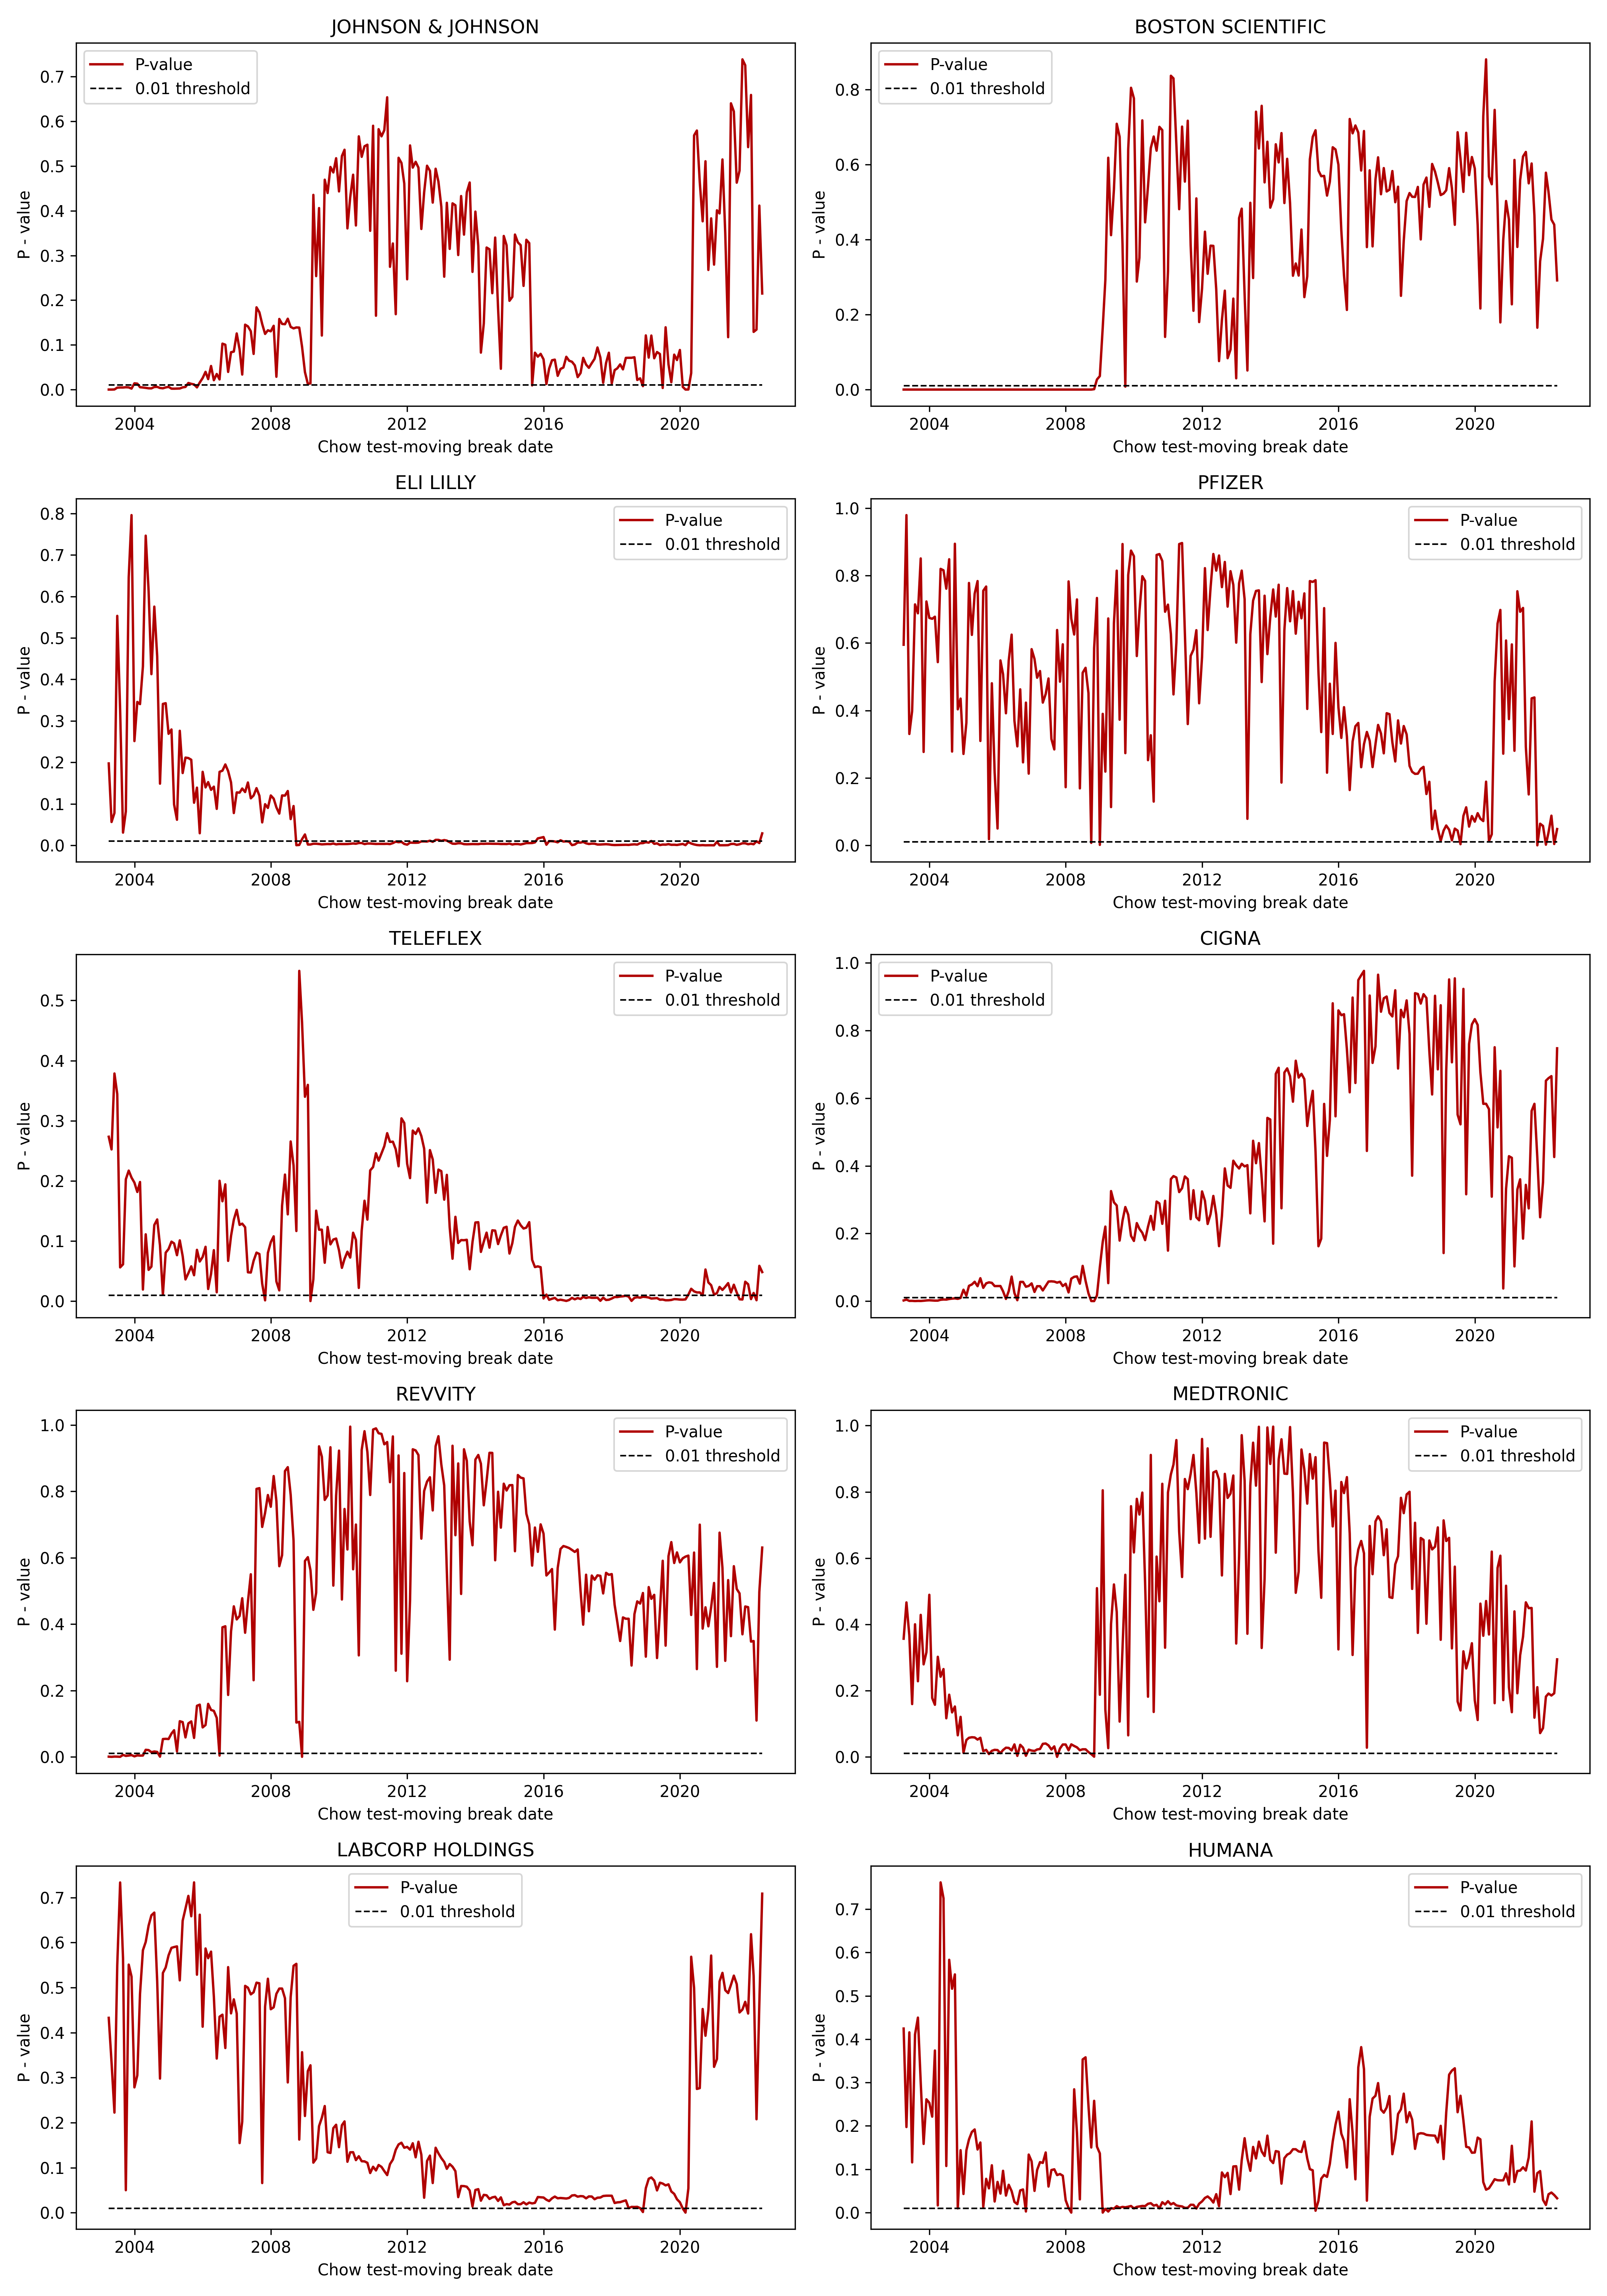
\includegraphics[width=0.8\textwidth]{images/chowmoving.png}
    \caption{Chow Test performed for all equities in search of structural breaks.}\label{fig:chowmoving}
\end{figure}

The results of this analysis are displayed in Figure~\ref{fig:chowmoving}, highlighting that different equities exhibit 
fundamentally distinct behaviors. 
Notably, certain equities, such as \textit{Eli Lilly}, \textit{Boston Scientific}, and \textit{Teleflex}, show p-values
consistently below the 0.01 threshold for extended periods, indicating prolonged structural breaks; this raises the question
of whether the CAPM relationship for these equities in these periods is truly linear or whether a different modeling approach
may be warranted.

\section{Periods of Shared Structural Breaks}

Despite these observations, no clear or consistent pattern of structural breaks emerges across all equities; to explore 
potential commonalities further, an additional histogram was generated (Figure~\ref{fig:struct_break_freqs}), which illustrates
the frequency and overlap of structural breaks shared among different equities.


\begin{figure}[h!]
    \centering
    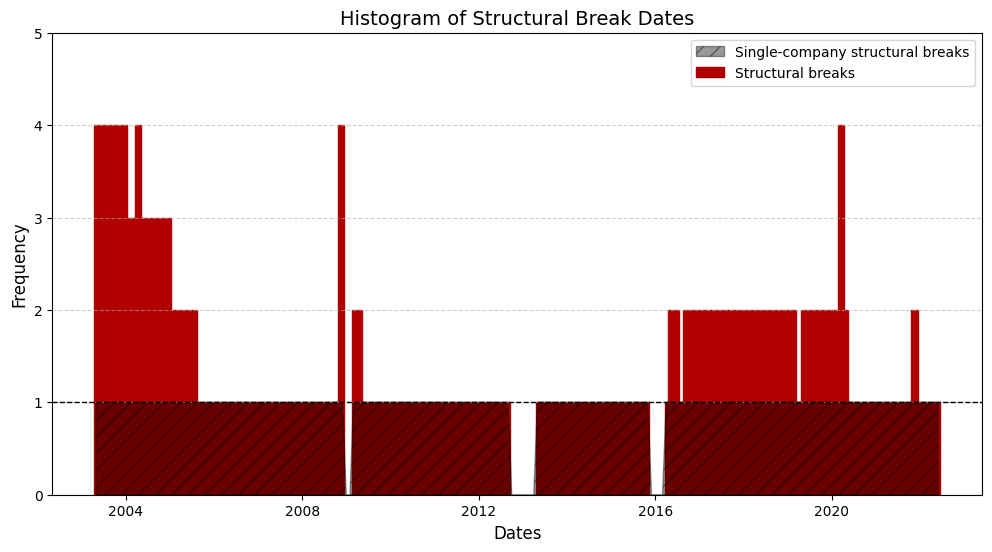
\includegraphics[width=0.8\textwidth]{images/struct_break_freqs.png}
    \caption{Frequency of months identified as structural break points.}\label{fig:struct_break_freqs}
\end{figure}

Figure~\ref{fig:struct_break_freqs} highlights two important aspects of the data: 
first, there is no single period that constitutes a break date for all equities, the maximum number of companies sharing a 
structural break at any given time is in fact 4; second, the identified break dates align closely with known economic and
market events.
Specifically, the data reveal three distinct periods of significant relevance, indicating concentrated structural breaks 
that may correspond to external shocks or sector-wide disruptions, those periods are:

\begin{enumerate}
    \item  \textbf{2003}: Structural breaks are observed throughout most of the year, coinciding with the SARS epidemic. 
    This period also aligns with economic and legislative developments, including the introduction of the Medicare
    Modernization Act, which reshaped healthcare policy and access in the United States.
    \item \textbf{October and November 2008}: These months mark the onset of the 2008/2009 financial crisis.
    \item \textbf{February and March 2020}: Structural breaks during this time correspond to the emergence of the COVID-19
    pandemic and the widespread implementation of precautionary measures.
\end{enumerate}

An important observation is that the structural breaks identified in 2003 extended over a prolonged period, spanning multiple
consecutive months, whereas the impact of the COVID-19 pandemic appears to have been more concentrated and shorter in duration
(see Figure~\ref{fig:struct_break_freqs}).
The prolonged effect in 2003 could reflect the gradual adjustment of the healthcare market to the SARS epidemic and concurrent
economic and legislative changes.
In contrast, the shorter duration of structural breaks during COVID-19 may indicate that advancements in epidemic preparedness,
such as improved healthcare infrastructure, rapid vaccine development, and the implementation of targeted government 
interventions, helped mitigate the impact of the pandemic on the healthcare market. 
Alternatively, the healthcare market may have simply grown so significantly in size and diversification over time that it 
developed a level of resilience that enables it to absorb and adapt to substantial disruptions in the economic landscape.
This explanation also accounts for the observation that, according to the Chow test, the majority of equities were not
significantly impacted during these events: the increased resilience and diversification of the healthcare market may have
allowed many companies to maintain stability despite the broader economic disruptions.
While these hypotheses provide potential explanations for the observed differences, a thorough investigation into these claims
is beyond the scope of this analysis.


\section{Chow Test on Portfolio}

In order to further investigate the impact of significant events in the economic environment, the same Chow test was 
performed on the excess returns of the portfolio. 
This approach aggregates the behavior of individual equities into a single measure, possibly allowing for the identification 
of systemic disruptions across the healthcare market.

\begin{figure}[h!]
    \centering
    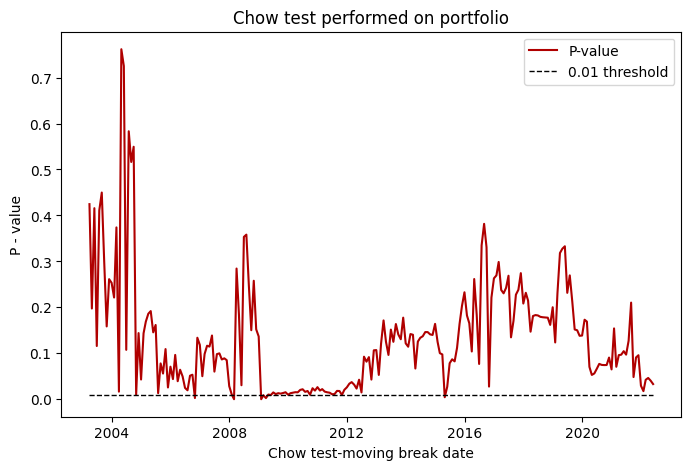
\includegraphics[width=0.8\textwidth]{images/portchowlio.png}
    \caption{Frequency of months identified as structural break points.}\label{fig:portchowlio}
\end{figure}

The results, displayed in Figure~\ref{fig:portchowlio}, show that the Chow test identifies a single time period with
particularly significant structural breaks in the portfolio's return dynamics: the beginning of 2009, likely reflecting the 
delayed impact of the 2008 financial crisis; this suggests that the crisis, while primarily affecting financial markets, 
also influenced the healthcare sector, albeit with a small lag.
Interestingly, the portfolio-level analysis contrasts with the results for individual equities, where multiple periods of 
structural breaks were observed.
Aggregating returns into a portfolio may have smoothed out smaller, company-specific disruptions, highlighting only the
most prominent systemic events.
Overall, the results emphasize that significant structural breaks in the healthcare market's portfolio-level returns are rare,
occurring primarily during periods of severe financial or economic crises.

%-------- Assignment 6 -----------------------------------------------------------------------------------------------------%
\chapter{Rolling CAPM Stability Analysis}\label{chapter:rolling}
\begin{figure}[h]
    \centering
    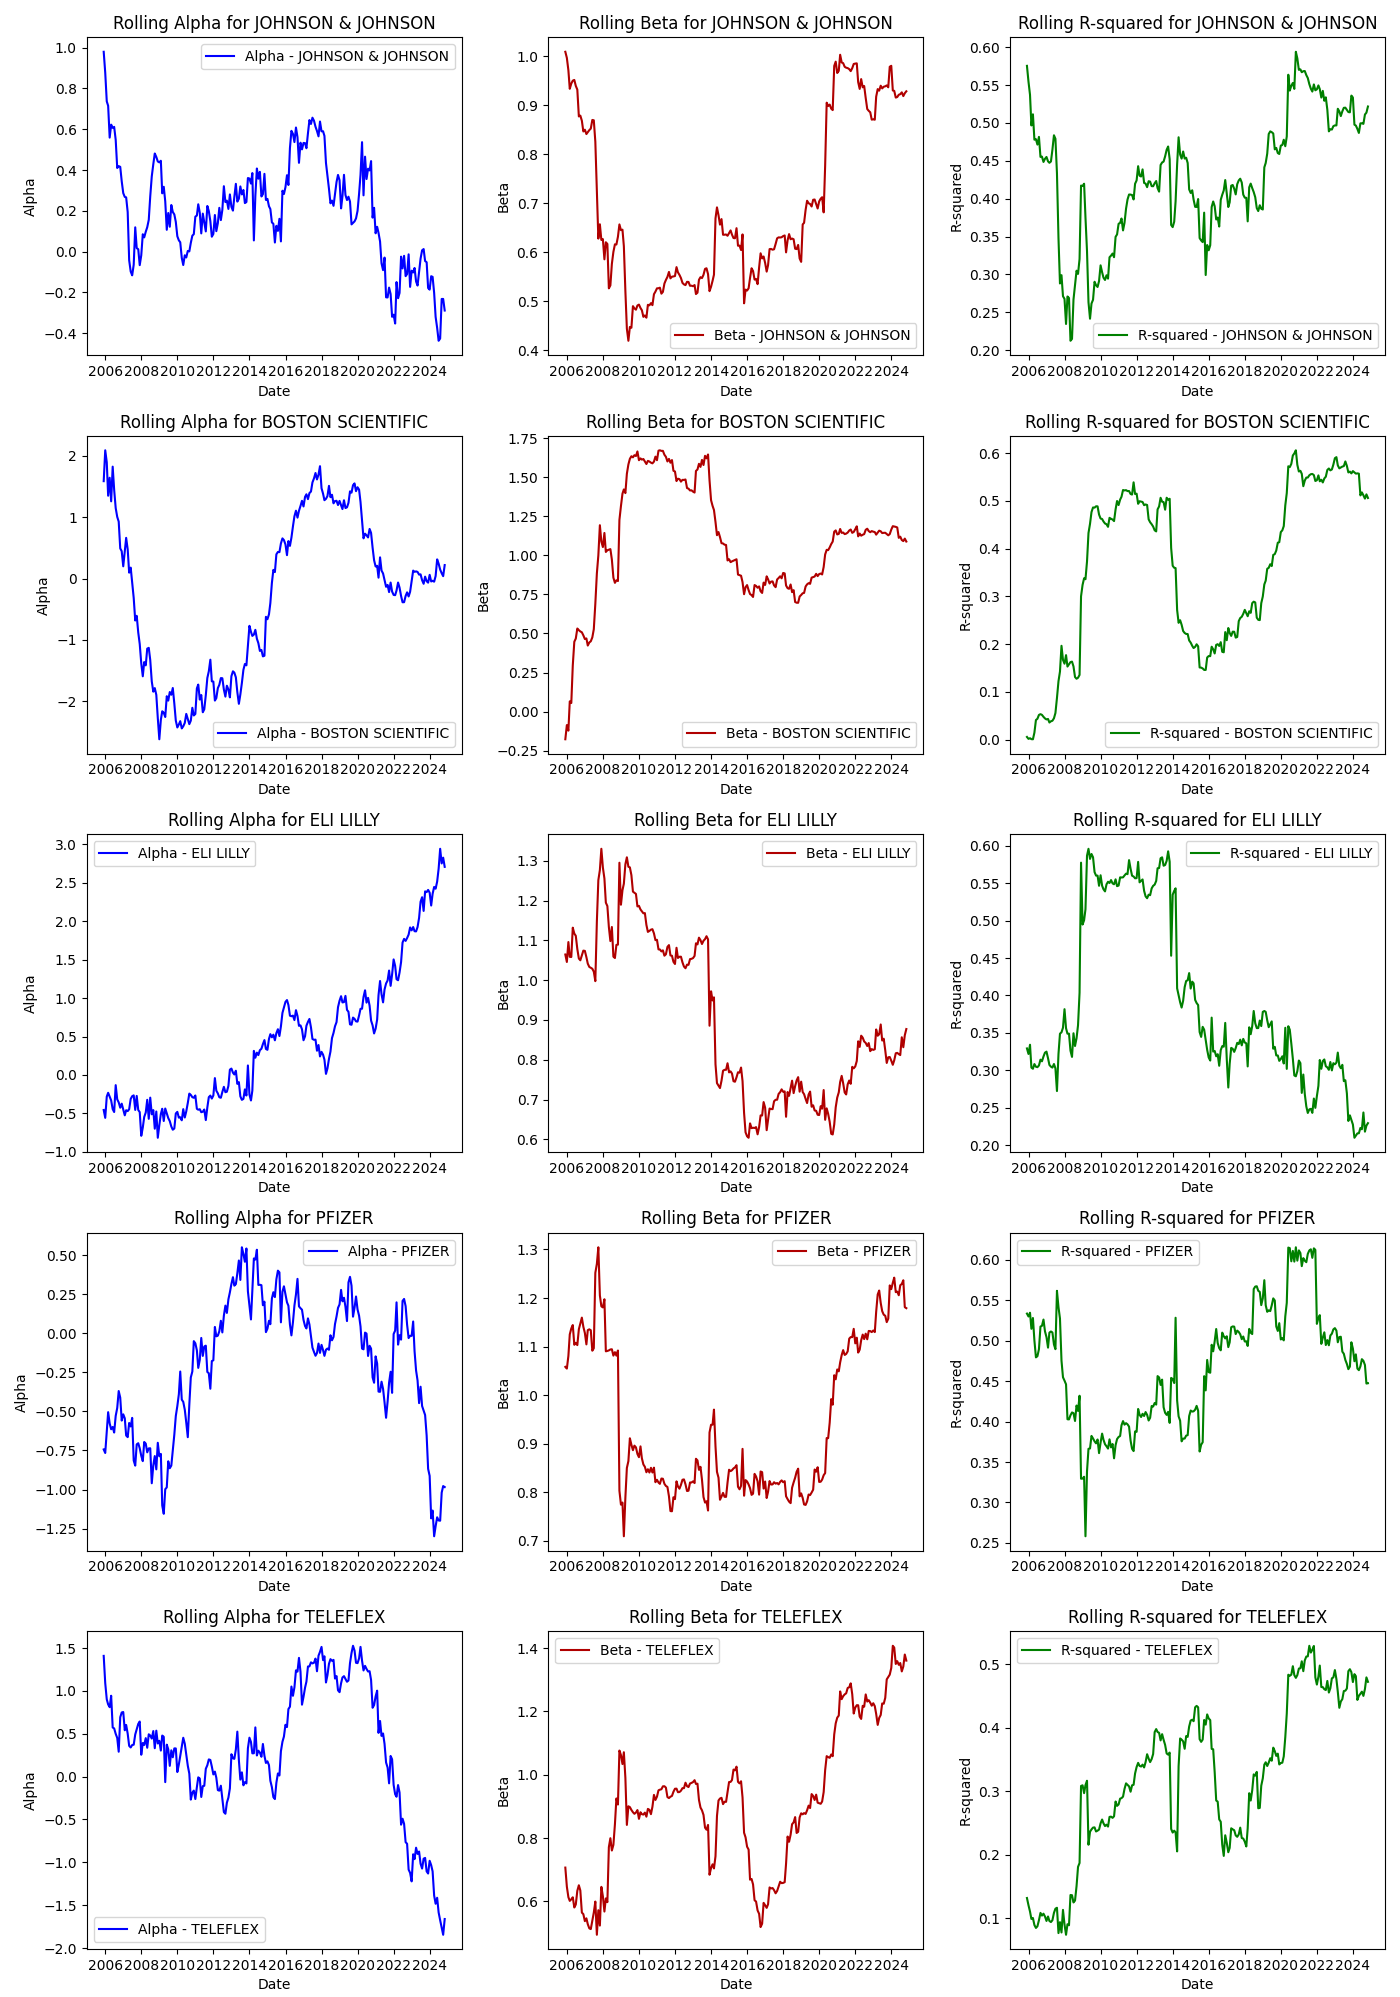
\includegraphics[width=0.8\textwidth]{images/rolling_quantities_1.png}
    \caption{Rolling quantities computed an all equities as an alternative of the Chow Test in search for structural
    breaks (1).}\label{fig:rolling_quantities_1}
\end{figure}
\begin{figure}[h]
    \centering
    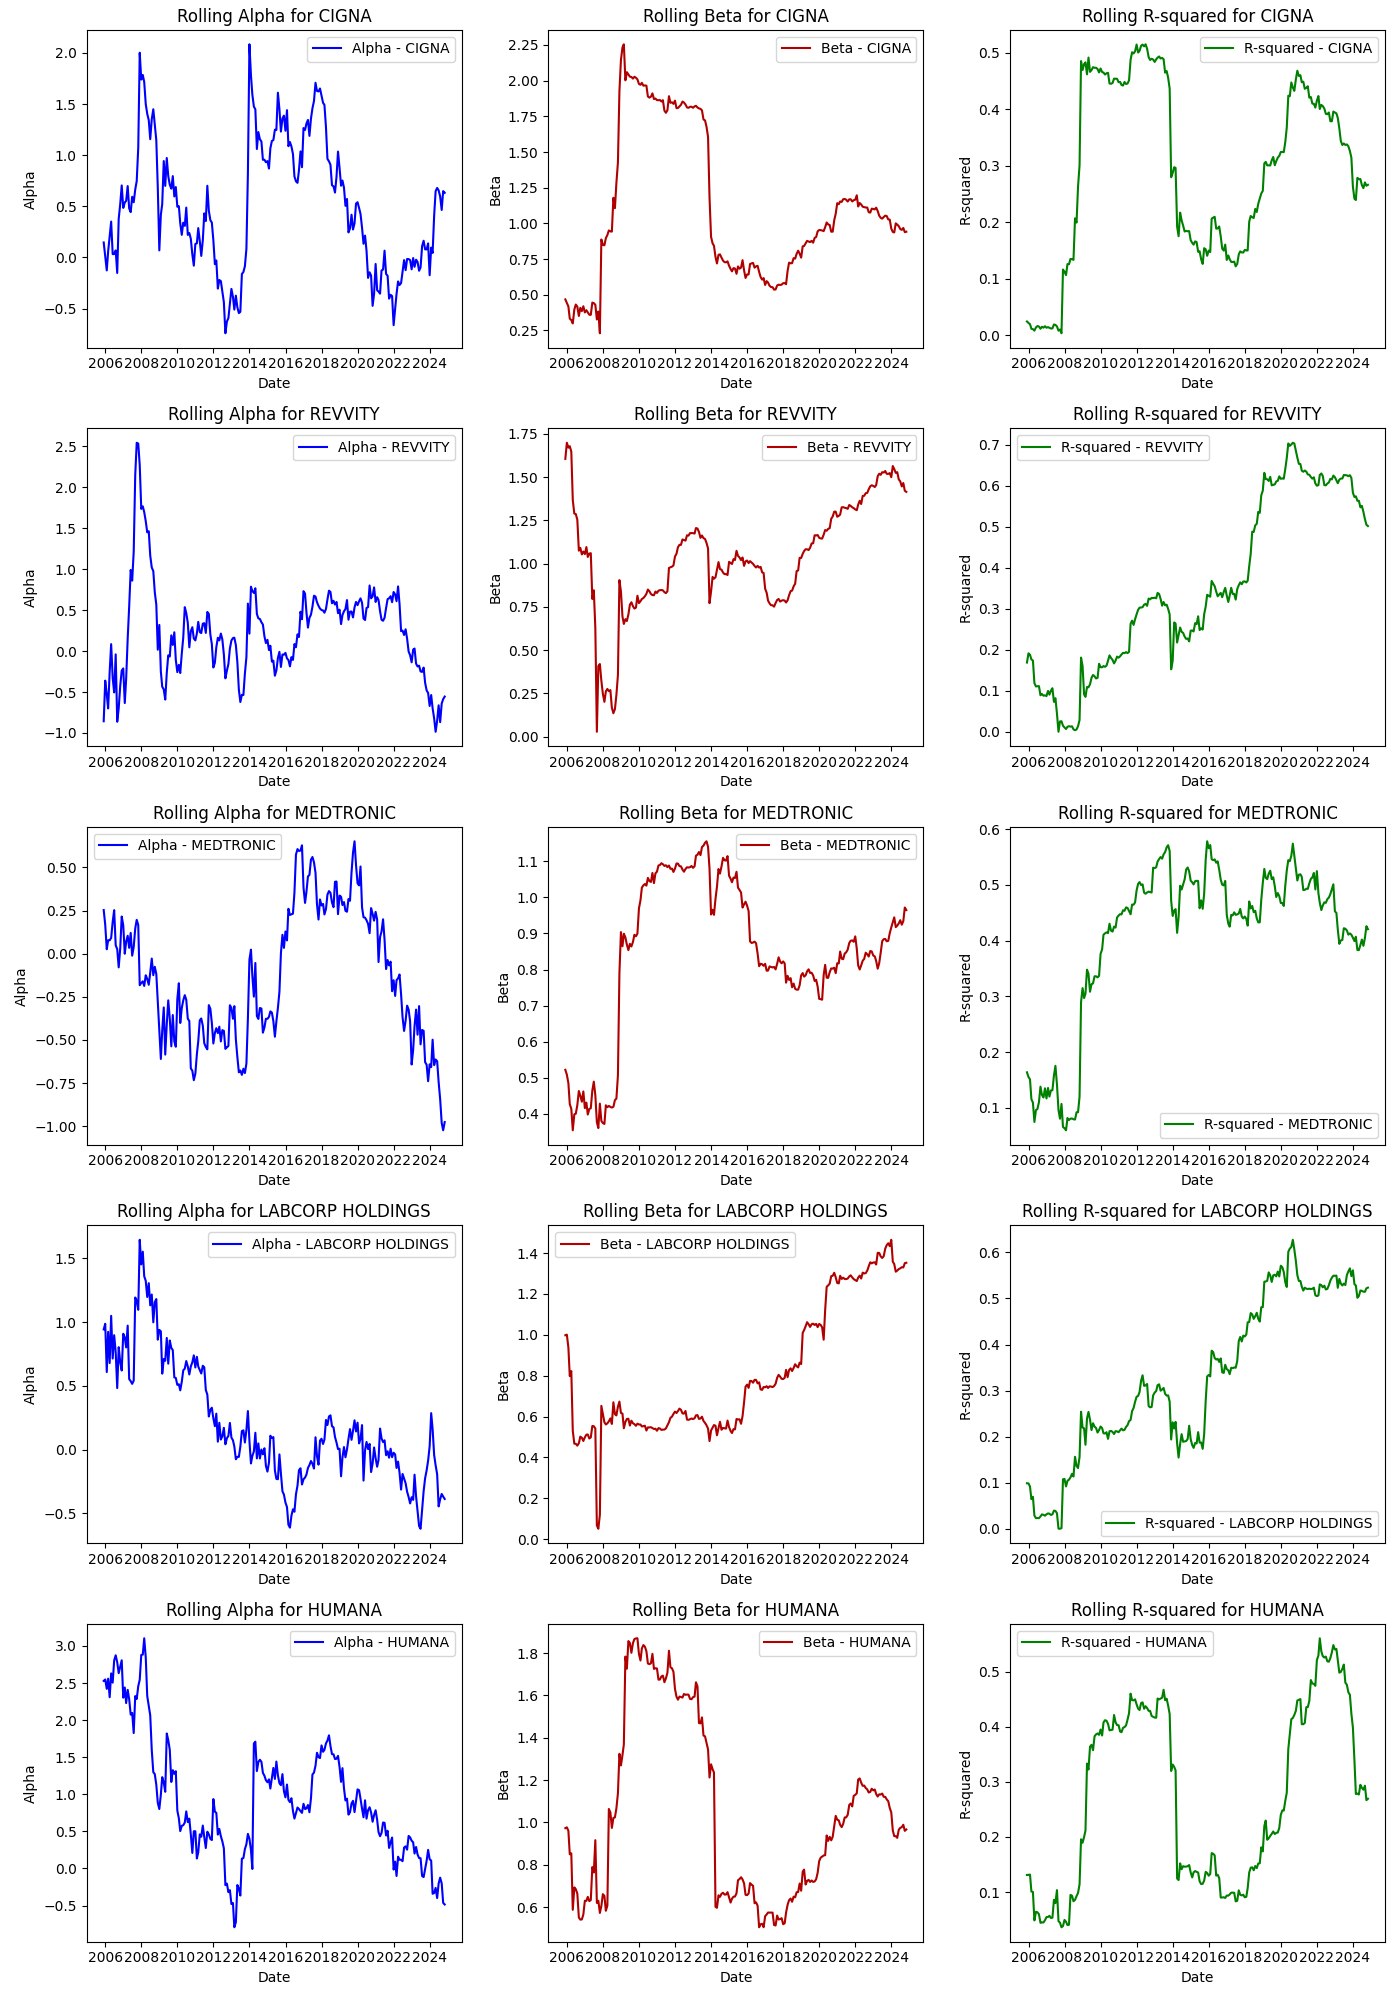
\includegraphics[width=0.8\textwidth]{images/rolling_quantities_2.png}
    \caption{Rolling quantities computed an all equities as an alternative of the Chow Test in search for structural
    breaks (2).}\label{fig:rolling_quantities_2}
\end{figure}


%-------- Assignment 7 -----------------------------------------------------------------------------------------------------%
\chapter{Multivariate Regression}\label{chapter:multivariate}

\begin{figure}[h]
    \centering
    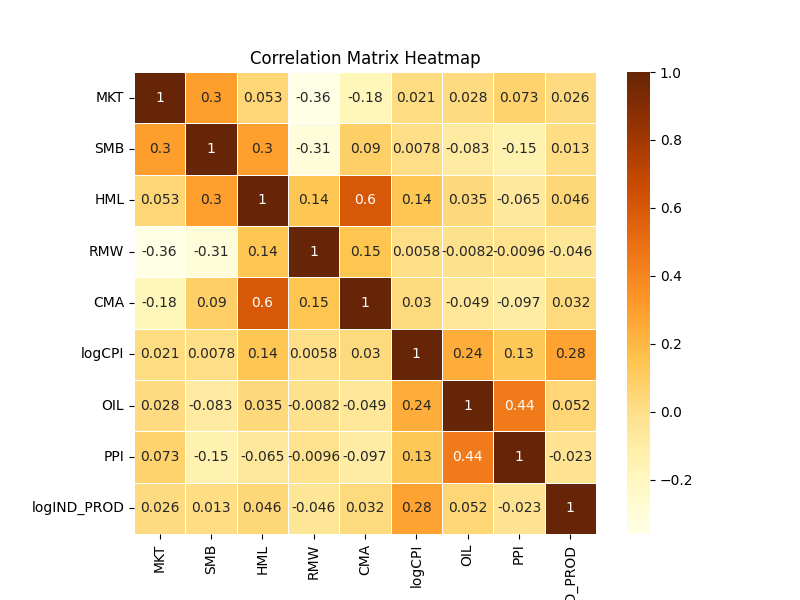
\includegraphics[width=0.8\textwidth]{images/Correlation_heatmap.png}
    \caption{Heatmap of the correlations between the chosen explainatory variables.}\label{fig:Correlation_heatmap}
\end{figure}

%-------- Appendix --------------------------------------------------------------------------------------------------------%
\chapter*{Appendix}\label{chapter:appendix}

%-------- GETS method -----------------------------------------------------------------------------------------------------%

\section*{Details of the GETS method}\label{section:GETS}

Here we present the outputs of the model developed using the GETS approach, which involves sequentially removing
statistically insignificant regression coefficients.

\begin{figure}[h!]
    \centering
    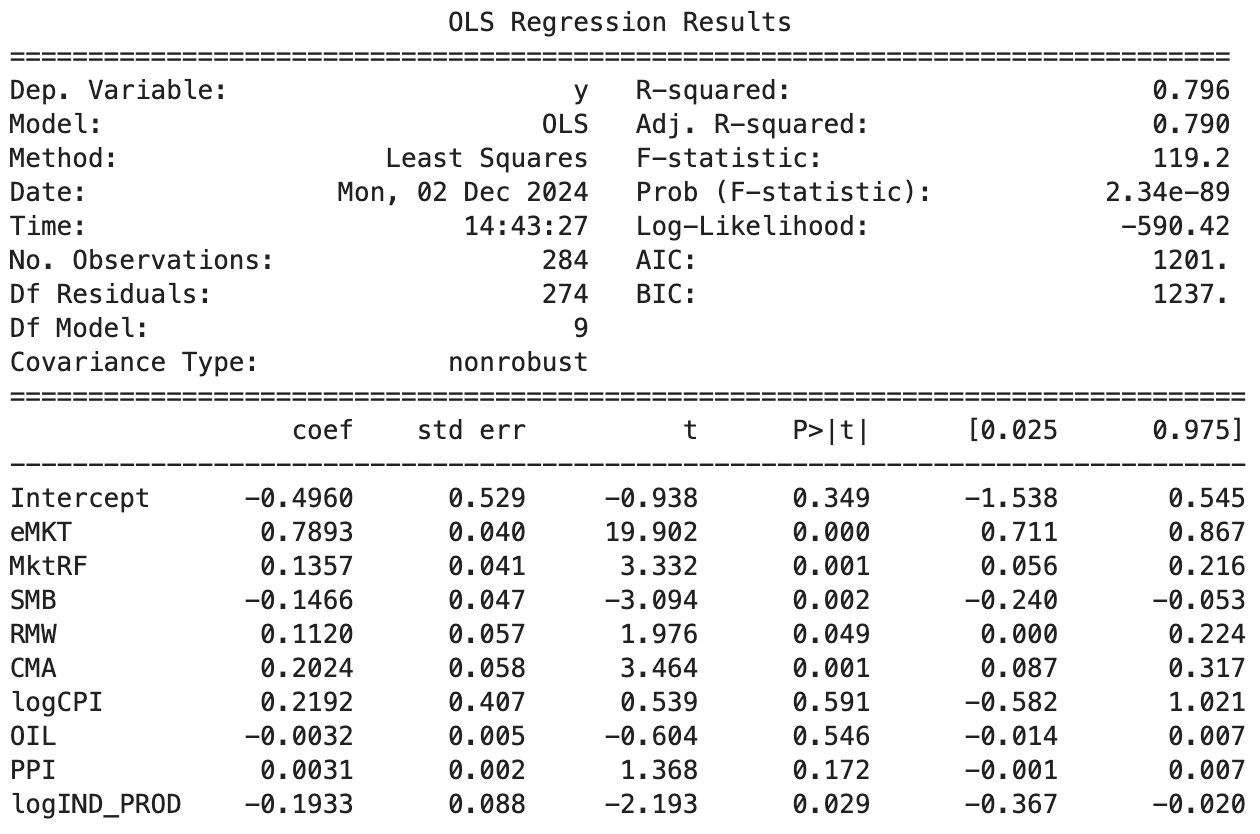
\includegraphics[width=0.8\textwidth]{images/HML1.png}
    \caption{Summary of the Regression after removing "HML"}\label{fig:HML1}
\end{figure} 

\begin{figure}[h!]
    \centering
    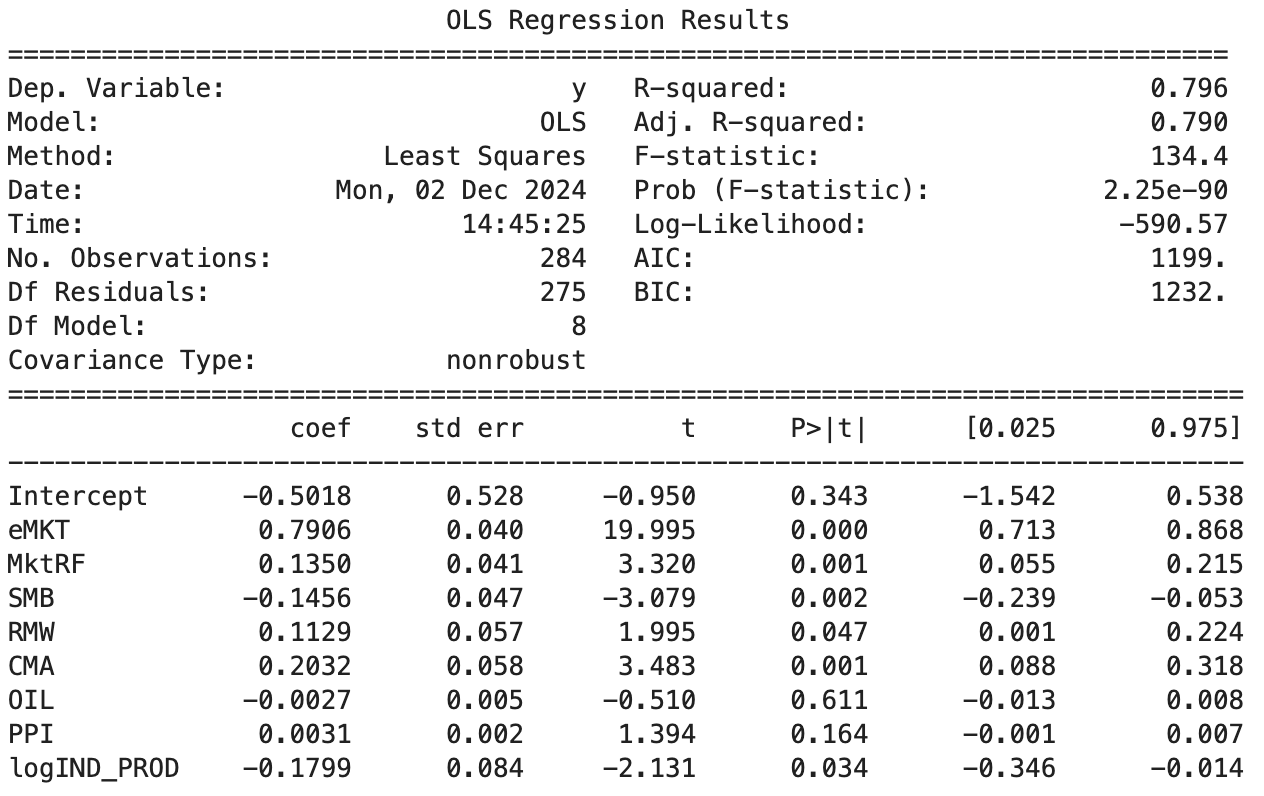
\includegraphics[width=0.8\textwidth]{images/LogCPI2.png}
    \caption{Summary of the Regression after removing "LogCPI".}\label{fig:CPI2}
\end{figure} 

\begin{figure}[h!]
    \centering
    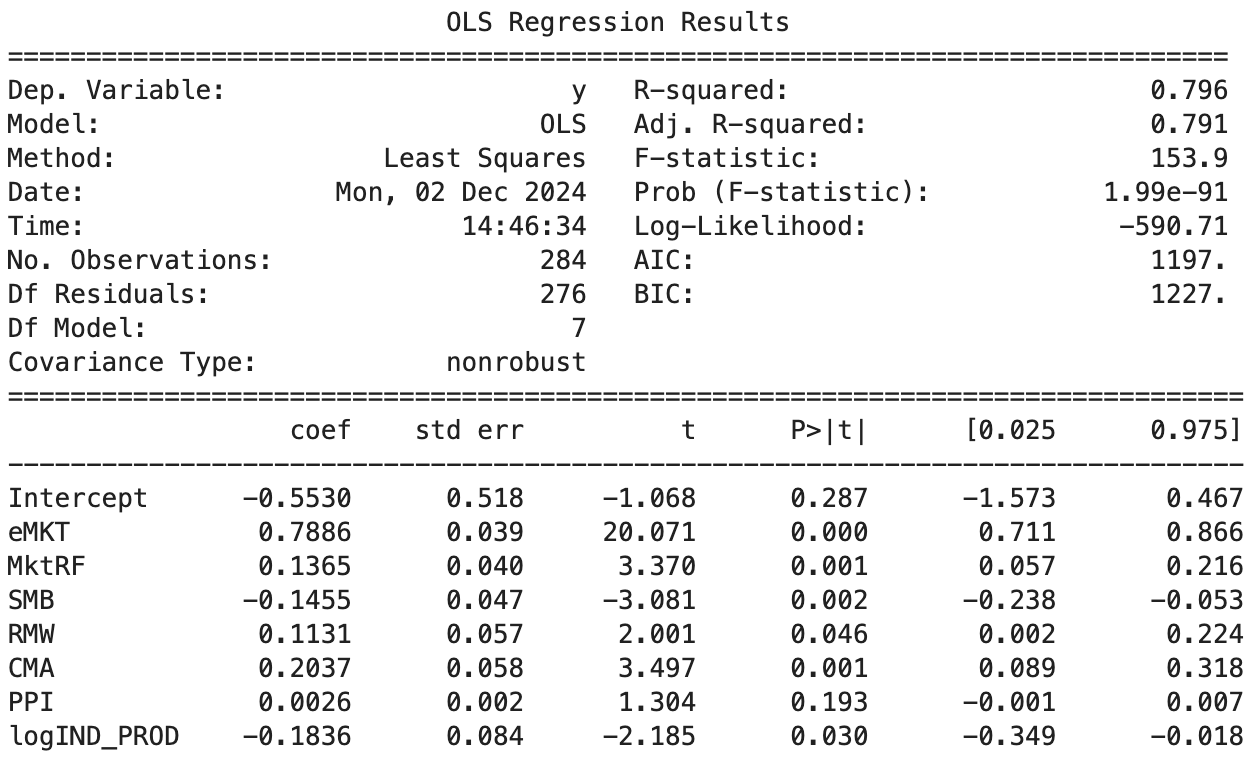
\includegraphics[width=0.8\textwidth]{images/OIL3.png}
    \caption{Summary of the Regression after removing "OIL".}\label{fig:OIL3}
\end{figure}
Figure~\ref{fig:PPI4} shows that the variable RMW has a p-value close to the 5\% threshold used as a benchmark for
determining whether to retain variables in the model. 

 \begin{figure}[h!]
    \centering
    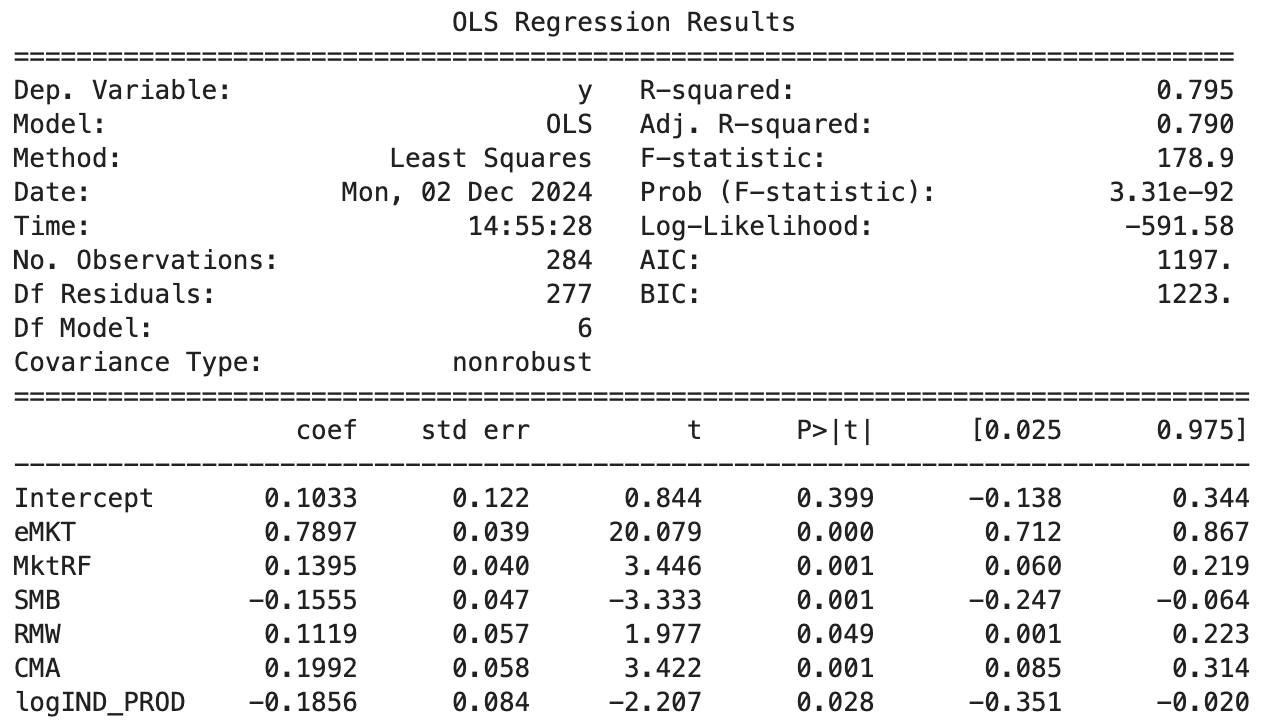
\includegraphics[width=0.8\textwidth]{images/PPI4.png}
    \caption{Summary of the Regression after removing "PPI".}\label{fig:PPI4}
\end{figure}

To assess its impact, we reran the model without RMW (Figure~\ref{fig:RMW5}) and observed a very small decrease in the 
adjusted $R^2$ (from 0.790 to 0.788).

\begin{figure}[h!]
    \centering
    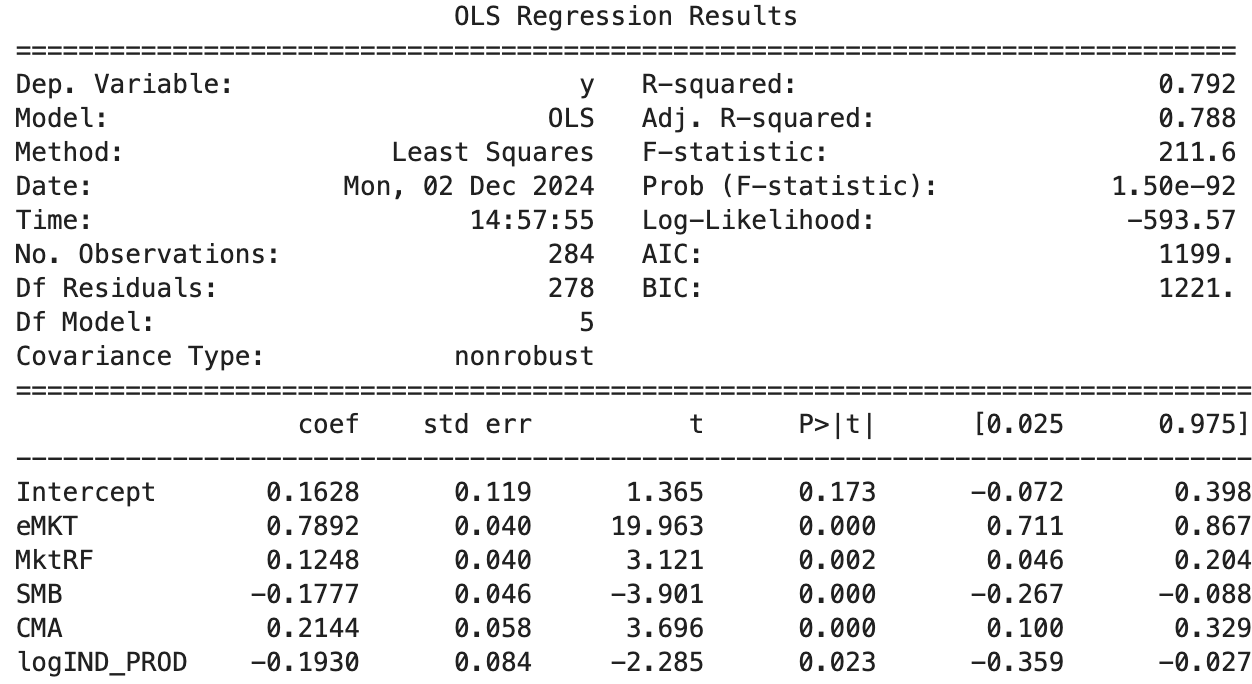
\includegraphics[width=0.8\textwidth]{images/RMW5.png}
    \caption{Summary of the Regression after removing "RMW".}\label{fig:RMW5}
\end{figure}


Given this minimal change in the prediction power and to adopt a more parsimonious model for the analysis, we decided to
exclude RMW from the regression.

%-------- Roles Summary ---------------------------------------------------------------------------------------------------%

\section*{Summary of Group Members' Contribution}

Table~\ref{tab:group_contribution} provides a detailed breakdown of each group member's contributions to the project. 
Notably, Giorgio Cottini also supervised the overall coding process and authored the accompanying LaTeX script.\\

\begin{table}[htbp]
    \centering
    \renewcommand{\arraystretch}{1.2} % Adjust row height
    \begin{tabular}{|c|l|l|}
        \hline
        \rowcolor{unired!40} \textbf{Assignment} & \textbf{Code}              & \textbf{Comment}         \\ \hline
        Assignment 1        & Enrico Paciaroni          & Enrico Paciaroni         \\ \hline
        \rowcolor{gray!10} Assignment 2        & Luigi Babiski             & Martina Arrighini        \\ \hline
        Assignment 3        & Giorgio Cottini           & Martina Arrighini        \\ \hline
        \rowcolor{gray!10} Assignment 4        & Martina Arrighini         & Martina Arrighini        \\ \hline
        Assignment 5        & Giorgio Cottini           & Giorgio Cottini          \\ \hline
        \rowcolor{gray!10} Assignment 6        & Luigi Babiski             & Luigi Babiski            \\ \hline
        Assignment 7        & Enrico Paciaroni          & Enrico Paciaroni         \\ \hline
    \end{tabular}
    \caption{Contribution of Group Members to Assignments}
    \label{tab:group_contribution}
\end{table}

%---------------------------------------------------------------------------------------------------------------------------%

\end{document}